\documentclass{article}
\usepackage{amsmath}
\usepackage{xcolor}
\usepackage{gensymb}
\usepackage{ragged2e}
\usepackage{graphicx}
\usepackage{gensymb}
\usepackage{mathtools}
\newcommand{\mydet}[1]{\ensuremath{\begin{vmatrix}#1\end{vmatrix}}}
\providecommand{\brak}[1]{\ensuremath{\left(#1\right)}}
\providecommand{\norm}[1]{\left\lVert#1\right\rVert}
\newcommand{\solution}{\noindent \textbf{Solution: }}
\newcommand{\myvec}[1]{\ensuremath{\begin{pmatrix}#1\end{pmatrix}}}
\let\vec\mathbf
\begin{document}
\begin{center}
        \textbf\large{CHAPTER-7 \\ TRIANGLES}
\end{center}
\section{Exercise 7.1}
Q1. In quadrilateral $CBAD$ as shon in figure \ref{fig:Fig}, \begin{equation} CA = AD \end{equation} and $BA$ bisect $\angle{A}$. Show that $\triangle{CAB} \cong \triangle{DAB}$. What can you say about $BC$ and $BD$? 
\\
\textbf{Construction}\\
The input parameters for construction:\\
\begin{tabular}{|p{3cm}|p{3cm}|p{3cm}|}
\hline                                        
\textbf{Symbol} & \textbf{Values} & \textbf{Description}\\                                          
\hline                                 
$\theta$ & 30$\degree{}$   & $\angle{BAD} = \angle{BAC}$ \\           
\hline                                    
a &  9 & $AB$ \\     
\hline                      
c & 5 & $AC$ \\
\hline                                     
		$\vec{e}_1$ & $\myvec{
			1\\
			0\\
			}$ & basis vector\\ 
\hline
\end{tabular}

\begin{align}
        A = \myvec{
                0\\        
                0\\        
                },
        B = \myvec{
                a\\
                0\\
                },
        C = \myvec{
                c.cos\theta\\
                c.sin\theta\\
                },
        D = \myvec{
                c.cos\theta\\
                -c.sin\theta\\
                }
\end{align}
\solution
\\
It is given that $AC$ and $AD$ are equal i.e., \begin{equation} CA = AD \end{equation} and the line segment $AB$ bisects $\angle{A}$.\\
\textbf{To Prove:}\\
The triangles $ACB$ and $ADB$ are similar i.e., \textbf{$\triangle{ACB} \cong \triangle{ADB}$}\\
\textbf{Proof:}\\
Consider the triangles $\triangle{CAB}$ and $\triangle{CAD}$
\begin{enumerate}
\item Now, consider equation of $AB$ as $y = 0$ which can be written as
	\begin{align}
                \vec{n}^{\top}X = 0
        \end{align} where
                \begin{align}
                        \vec{X} = \myvec{
                                  x\\
                                  y\\
                                  },
                        \vec{n} = \myvec{
                                  0\\
                                  1\\
                                  }
                \end{align}
\item Next, we can consider the vertex $B$ as
        \begin{align}
                B = a(e1)
        \end{align} where
        \begin{align}
                \vec{e1}=\myvec{
                        1\\
                        0\\
                        }
        \end{align}
\item From the above assumptions, we get the coordinates of $C$ and $D$ as
        \begin{align}
                \vec{C} = \myvec{
                        c cos\theta\\
                        c sin\theta\\
                        }
                \vec{D} = \myvec{
                        c cos\theta\\
                        -c sin\theta\\
                        }
        \end{align}
\item Finding the angles(according to assumptions):
        \begin{align}
		cos\angle{CBA} = \frac{(B-C)^\top(B-A)}{\norm{B-C}\norm{B-A}}\\
        \implies \vec{((B-C)^\top)(B-A)} &= \myvec{
                                         9-5 cos30\degree{}\\
                                         -5 sin30\degree{}\\
                                        }^\top \cdot \myvec{
                                                        9\\
                                                        0\\
                                                        }\\
                        &= 9^2-9.5.cos30\degree{}-9.5.sin30\degree{}\\
			&= 81-45(\frac{1+\sqrt{3}}{2})\\
        \implies \norm{B-C}\norm{B-A} &= (\sqrt{(9-5.cos30\degree{})^2+(-5.sin30\degree{})^2})(9)\\
                        &= (\sqrt{9^2+5^2-2.9.5.cos30\degree{}})(9)\\
			&= 9\sqrt{106-45\sqrt{3}}\\
        \end{align}
		From equations (12) and (14), \begin{align} cos\angle{CBA} &= \frac{9-5.cos30\degree{}-5.sin30\degree{}}{\sqrt{9^2+5^2-2.9.5.cos30\degree{}}}\\
		&= 65.8\degree{}\\ \end{align}
        \begin{align}
		cos\angle{ABD} = \frac{(B-D)^\top(B-A)}{\norm{B-D}\norm{B-A}}\\
	Put \theta as -\theta in above equation\\
        \implies \vec{((B-D)^\top)(B-A)} &= \myvec{
					9-5 cos(-30)\degree{}\\
					5 sin(-30)\degree{}\\
                                       }^\top \cdot \myvec{
                                                        9\\
                                                        0\\
                                                        }\\
			&= 9^2-9.5.cos(-30)\degree{}+9.5.sin(-30)\degree{}\\
			&= 81-45(\frac{\sqrt{3}+1}{2})\\
		\implies \norm{B-D}\norm{B-A} &= (\sqrt{(9-5.cos(-30)\degree{})^2+(5.sin(-30)\degree{})^2})(9)\\
			&= (\sqrt{9^2+5^2-2.9.5.cos(-30)\degree{}})(9)\\
			&= 9\sqrt{106-45\sqrt{3}}\\
	\end{align}
From equations (18) and (20), 
\begin{align}
	cos\angle{ABD} &= \frac{9-5.cos30\degree{}+5.sin30\degree{}}{\sqrt{9^2+5^2-2.9.5.cos30\degree{}}}\\
		       &= 65.8\\
                       &= cos\angle{CBA}\\
\end{align}
\item We know that sum of the angles in a triangle is 180\degree{} ,
\begin{align}
	\angle{BAC} & = 180\degree{} - \angle{CBA} - \angle{BCA}\\
		    & = 180\degree{} - \angle{ABD} - \angle{DCA} \\
		    & = 180\degree{} - 65.8\degree{} -30\degree{}\\
		    & = 84.2\degree{} \text{ (From Eq.21 and given) }
\end{align}
Since all the angles and sides of triangles $CAB$ and $CAD$ are equal , from the definition of congruency both the triangles are said to be congruent to each other.
\begin{align}
        \triangle{CAB} & \cong \triangle{CAD}\\
        AB &= AD 
\end{align}
\begin{figure}
	\begin{center}
		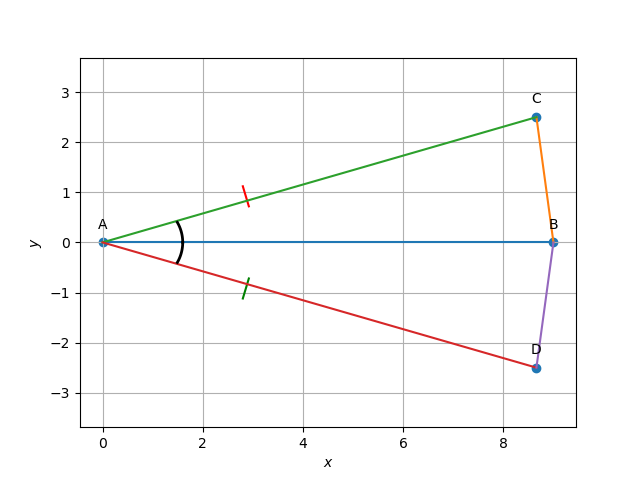
\includegraphics[width=\columnwidth]{figs/graph.png}
		\caption{Quadrilateral CBAD}
		\label{fig:Fig}
	\end{center}
\end{figure}
\end{enumerate}
\end{document} 
